	\documentclass[10pt,oneside]{CBFT_book}
	% Algunos paquetes
	\usepackage{amssymb}
	\usepackage{amsmath}
	\usepackage{graphicx}
% 	\usepackage{libertine}
% 	\usepackage[bold-style=TeX]{unicode-math}
	\usepackage{lipsum}

	\usepackage{natbib}
	\setcitestyle{square}

	\usepackage{polyglossia}
	\setdefaultlanguage{spanish}


	\usepackage{CBFT.estilo} % Cargo la hoja de estilo

	% Tipografías
	% \setromanfont[Mapping=tex-text]{Linux Libertine O}
	% \setsansfont[Mapping=tex-text]{DejaVu Sans}
	% \setmonofont[Mapping=tex-text]{DejaVu Sans Mono}

	%===================================================================
	%	DOCUMENTO PROPIAMENTE DICHO
	%===================================================================

\begin{document}

% =================================================================================================
\chapter{Relatividad especial}
% =================================================================================================

% =================================================================================================
\section{Transformación de vectores}
% =================================================================================================

Digamos que un vector transforma 
\[
	X'_{i} = a_{ij} X_j
\]
de manera que se verifique que las leyes físicas sean invariantes frente a rotaciones propias.
El módulo no cambia $ |\vb{X}'|^ 2 = |\vb{X}|^2$.

Einstein postula que:
\begin{itemize}
 \item Todos los sistemas inerciales son equivalentes (no se puede hablar de espacio absoluto).
 \item La velocidad de la luz en un sistema inercial es constante. No depende del estado de
 movimiento del observador.
\end{itemize}



Las ecuaciones vistas hasta ahora son igualdades vectoriales.
Toda ley física debe ser covariante de un sistema inercial a otro.

Para una magnitud tensorial de 2do rango la traza del mismo debe ser invariante y además satisface
\[
	a_{ij} a_{ik} = \delta_{jk}.
\]
Transformación ortogonal.
En la época de Maxwell se postuló que las ondas EM viajaban con velocidad $c$ respecto al espacio absoluto
(el éter). Pero esta idea muere con Einstein en 1905.

Sea un sistema $S'$ que se mueve con velocidad \vb{v} de otro $S$ en forma paralela a un eje (ver figura).
\begin{figure}[htb]
	\begin{center}
	\includegraphics[width=0.4\textwidth]{images/fig_ft1_transfvec.pdf}	 
	\end{center}
	\caption{}
\end{figure}

Se verifica entonces la transformación de Lorentz
\begin{align*}
	x^{1'} &= x^1  \\
	x^{2'} &= x^2  \\
	x^{3'} &= \gamma \: [ x^3 - \beta x^0]  \\
	x^{0'} &= \gamma \: [ x^0 - \beta x^3] 
\end{align*}
donde son 
\[
	\gamma = \frac{1}{(1 - v^2/c^2)^{1/2}} \qquad \qquad x^0 = ct 
\]

A la transformación [1] se le puede dar forma de rotación en funciones hiperbólicas como sigue
definiendo
\[
	\beta \equiv \tanh(\eta) \qquad \gamma \equiv \cosh(\eta) \qquad 
	\gamma\cdot \beta = \sinh(\eta)
\]
y con esta nueva notación puede escribirse
\[
	x^{0'} = x^0 \cosh( \eta ) - x^3 \sinh( \eta )
\]
\[
	x^{3'} = -x^0 \sinh( \eta ) + x^3 \cosh( \eta )
\]
donde seguimos viendo que las leyes son lineales en las coordenadas (el espacio es isótropo)
\notamargen{Debiéramos dar ideas de estas cosas importantes de relatividad especial}
\[
	\begin{pmatrix}
	 x^{0'} \\
	 x^{3'} \\
	\end{pmatrix}
	=
	\begin{pmatrix}
	\cosh( \eta ) & \sinh( \eta ) \\
	-\sinh( \eta ) & \cosh( \eta ) \\
	\end{pmatrix}
	\begin{pmatrix}
	 x^{0} \\
	 x^{3} \\
	\end{pmatrix}
\]
y no es otra cosa  que una rotación en eje $\hat{0}, \hat{3}$ con el ángulo $\eta = \atanh( \beta )$.
O sea, son rotaciones en funciones hiperbólicas.
Notemos que se verifica la invariancia del módulo de la transformación
\[
	(x^{0'})^2 -  ( (x^{1'})^2  + (x^{2'})^2 + (x^{3'})^2 ) =
		(x^{0})^2 -  ( (x^{1})^2  + (x^{2})^2 + (x^{3})^2 ) 
\]
o en una notación más feliz
\[
	(ct')^2 - ( x'^2 + y'^2 + z'^2 ) = (ct)^2 - ( x^2 + y^2 + z^2 )
\]
Estamos queriendo generar una estructura geométrica para pasar entre sistemas inerciales.

	
Este espacio 4D es el de Minkowski y no es euclídeo.
Un punto de este espacio es lo que se llama un {\it evento}; el radio vector posición en
este espacio.

Busquemos ahora la transformación inversa. Dado que
\[
	\begin{cases}
	x^{0'} = \gamma (x^0 - \beta x^3) \\
	\\
	x^{3'} = \gamma (x^3 - \beta x^0)
	\end{cases}
\]
y entonces se tienen los componentes contravariantes de las coordenadas del evento,
que verifican
\[
	\begin{pmatrix}
	 x^{0'} \\
	 x^{1'} \\
	 x^{2'} \\
	 x^{3'} \\
	\end{pmatrix}
	=
	\begin{pmatrix}
	\gamma & 0 & 0 & -\beta\gamma \\
	0 & 1 & 0 & 0 \\
	0 & 0 & 1 & 0\\
	-\beta\gamma  & 0 & 0 & \gamma \\
	\end{pmatrix}
	\begin{pmatrix}
	 x^{0} \\
	 x^{1} \\
	 x^{2} \\
	 x^{3} \\
	\end{pmatrix}
\]
y la transformación inversa, que se obtiene tomando los reemplazos
\[
	x^{i'} \to x^i \quad ,\quad  x^i \to x^{i'} \quad ,\quad  \beta \to -\beta,
\]
permite hallar los componentes covariantes de dichas coordenadas que verifican
\[
	\begin{pmatrix}
	 x^{0} \\
	 x^{1} \\
	 x^{2} \\
	 x^{3} \\
	\end{pmatrix}
	=
	\begin{pmatrix}
	\gamma & 0 & 0 & \beta\gamma \\
	0 & 1 & 0 & 0 \\
	0 & 0 & 1 & 0\\
	\beta\gamma  & 0 & 0 & \gamma \\
	\end{pmatrix}
	\begin{pmatrix}
	 x^{0'} \\
	 x^{1'} \\
	 x^{2'} \\
	 x^{3'} \\
	\end{pmatrix}
\]

En realidad hemos considerado una transformación de Lorentz muy sencilla. Una 
más general será
\[
	\begin{cases}
	x^{\alpha'} = x^{\alpha'}(x^0, x^1, x^2, x^3) \\
	\\
	x^{\alpha} = x^{\alpha}(x^{0'}, x^{1'}, x^{2'}, x^{3'})
	\end{cases}
\]
que nos da el radio vector contravariante y el covariante, respectivamente.
Cada coordenada es función de todas las otras.


El elemento diferencial de línea, que es un invariante, es 
\[
	ds^2 = (dx^0)^2 - (dx^1)^2 - (dx^2)^2 - (dx^3)^2 = ds^{'2}
\]
o bien 
\[
	ds^2 = g_{\alpha\beta}dx^{\alpha}dx^{\beta}
\]
que define el tensor de la métrica. Se verifica
\[
	g_{\alpha\beta} = g^{\alpha\beta} =
	\begin{pmatrix}
	 1 & 0 & 0 & 0 \\
	 0 & -1 & 0 & 0 \\
	 0 & 0 & -1 & 0 \\
	 0 & 0 & 0 & -1 \\
	\end{pmatrix}
\]

\subsubsection{Cuadrivectores en el espacio 4D}

Un cuadrivector contravariante es
\[
	A^{\mu} = ( A^0, \vb{A})
\]
mientras que el covariante es
\[
	A_{\mu} = ( A^0, -\vb{A})
\]
y vemos que las partes temporales son las mismas cambiando el signo de la espacial. Las reglas de 
transformación son
\[
	A'^{\alpha}= \dpar{x'^{\alpha}}{x^{\beta}} A^{\beta} \qquad\qquad 
		A'_{\alpha}= \dpar{x^{\beta}}{x'^{\alpha}} A_{\beta}
\]
luego el producto interno es
\[
	\widetilde{A}\cdot\widetilde{B} \equiv A_\alpha B^\alpha
\]
donde estamos usando convención de suma de Einstein, que significa que 
\[
	\widetilde{A}\cdot\widetilde{B} = A^0 B^0 -\pe{A}{B}
\]
que es invariante por ser un escalar de Lorentz,
\[
	A_\alpha B^\alpha = A'_\alpha B'^\alpha
\]

Se ve que las reglas de transformación son tales que en el producto interno se cancelan los factores
y el mismo resulta, como es sano que suceda, independiente del sistema coordenado.
No cualesquiera cuatro cantidades forman los componentes de un cuadrivector.

\subsubsection{Intervalos entre eventos}

La distancia entre evento origen y un evento cualquiera es
\[
	S^2 = g_{\alpha\beta} X^\alpha X^\beta = (ct)^2 - (x^1)^2 - (x^2)^2 - (x^3)^2,
\]
pero los intervalos deben ser invariantes relativistas y de Lorentz.
Si el intervalo es temporal se tiene 
\[
	x^0 > x^i x_i \Rightarrow \delta s^2 > 0  
\]
y los eventos pueden estar conectados causalmente
\[
	x^0 < x^i x_i \Rightarrow \delta s^2 < 0 
\]
y los eventos no pueden estar conectados causalmente. Se cumple
\[
	\delta s^2 = (x^0)^2 - [ (x^1)^2 + (x^2)^2 + (x^3)^2 ]
\]

Como $\delta s^2$ es un invariante, entonces el carácter del mismo se conserva en todos
los sistemas inerciales.

\subsubsection{Operadores diferenciales}

Tenemos la derivada respecto a una coordenada contravariante
\[
	\partial_\alpha \equiv \dpar{}{x^\alpha} = \left( \dpar{}{x^0}, \Nabla \right)
\]
que es la derivada covariante, y también la derivada respecto de una coordenada covariante
\[
	\partial^\alpha \equiv \dpar{}{x_\alpha} = \left( \dpar{}{x^0}, - \Nabla \right)
\]
que es la derivada contravariante. Note la asimetría entre derivo respecto de arriba y es derivada abajo
y viceversa. La notación abreviada puede inducir a confusiones.
\notamargen{En el operador $\partial_{\alpha}$ el subíndice cambia de ubicación pero se mantiene el
caracter (contra-) o (co-) variante del operador.}

La cuadridivergencia de un cuadrivector es un invariante,
\[
	\partial_\alpha A^\alpha = \dpar{A^0}{x^0} + \Nabla\cdot\vb{A}
\]
\[
	\partial^\alpha A_\alpha = \dpar{A^0}{x^0} - \Nabla\cdot(-\vb{A})
\]
y aquí vemos $\partial_\alpha A^\alpha = \partial^\alpha A_\alpha$. Esto nos lleva al D'Alembertiano
\[
	\Box \equiv \partial_\alpha \partial^\alpha = \dpar[2]{}{x^0} - \nabla^2
\]

{\bf Conexión de sucesos}

Sean dos sucesos $x_1^\alpha, x_2^\alpha$ tales que 
$s^2$ es el intervalo entre los mismos (al cuadrado), y es un invariante lorentziano
\[
	s^2 = c^2( t_1 - t_2 )^2 - | \vb{x}_1 - \vb{x}_2 |^2
\]
El intervalo es temporal si $s^2 >0$ en cuyo caso se tiene 
\[
	c \delta t >  | \vb{x}_1 - \vb{x}_2 |
\]
lo cual significa que existe frame inercial donde $x_1=x_2$ los eventos ocurren en el mismo sitio de manera
que pueden estar conectados causalmente; puesto que $c\delta t > 0$ y $t_2>t_1$. Por el contrario si 
$c^2 < 0$ se tiene 
\[
	c \delta t <  | \vb{x}_1 - \vb{x}_2 |
\]
y existe entonces frame inercial donde los dos eventos son en el mismo sitio $x_1=x_2$ y entonces $c\delta t 
< 0$ y $t_2 < t_1$ de manera que no pueden estar conectados causalmente.

Sea 
\[
	dt'= \gamma \left( dt - \frac{v}{c^2} dz \right)
\]
y si es $\textcircled{2}$ posterior a $\textcircled{1}$ en $S$ entonces $dt > 0 $.
Entonces $ dt'$ puede ser mayor, menor o igual a cero (no respeta la temporalidad de $S$).

El orden temporal se puede alterar pasando de $S$ a $S'$, pero en ese caso se rompe la causalidad.
En todos aquellos intervalos donde tienen diferentes signos $dt$ y $dt'$ se viola el principio de causalidad.
Dos sucesos estarán relacionados causalmente si dado $dt > 0$ se tiene 
\[
	dt > \frac{v}{c^2} dz
\]
y eligiendo $S'$ fijo a la señal que se emite y siendo $v$ la velocidad de propagación de la señal, será
\[
	1 > \frac{v}{c^2} \dtot{z}{t} = \frac{v^2}{c^2}
\]
para que ninguna señal se pueda mover a mayor velocidad que la de la luz (porque tiene que valer la
causalidad).
El gráfico siguiente intenta ilustrar estas consideraciones.
Suponemos haz de luz desde el $-\infty$ que pasa por el origen

\begin{figure}[htb]
	\begin{center}
	\includegraphics[width=0.7\textwidth]{images/fig_ft1_intervalos.pdf}	 
	\end{center}
	\caption{}
\end{figure} 

Ahora se ve lo que pasa para otro observador haciendo un cambio de coordenadas 
\[
	x'^0 = \gamma (x^0 - \beta x^3) \qquad x'^3 = \gamma (x^3 - \beta x^0)
\]
y si ahora es $x'^0 = 0$ entonces para un observador en $S'$ se tiene 
\[
	0 = \gamma (x^0 - \beta x^3) 
\]
o bien $x^0 = \beta x^3$ y aquí es $x'^3 = 0$ de modo que 
\[
	\frac{x^3}{\beta} = x^0
\]
y entonces $a$ de la figura puede ser causado por un suceso en el origen pero $b$ no tiene 
conexión causal con el origen.

Para el observador $S'$ el punto $b$ está debajo de su ``ahora'' que es el pasado.
Por otra parte $a$ para el observador S es el futuro. Para este mismo observador, el punto
$b$ está en ``cualquier otra parte'' de tal manera que no puede estar conectado causalmente
con el origen.

\begin{ejemplo}{\bf Problema}
 
No relativista será la información propia (desde el sistema donde se produce el evento solidario
al objeto). Tenemos $K, K'$ sistemas inerciales, donde el segundo se mueve con velocidad \vb{V}
con respecto al primero. Suponemos $\vb{V} = V\zver$.
\[
	\xver \parallel \xver' \qquad 
	\yver \parallel \yver' \qquad 
	\zver \parallel \zver'
\]
Una barra moviéndose en $K'$ a velocidad constante medida desde $K$
\[
	\begin{cases}
		L'= Z_1'- Z'_0 \\
		L= Z_1- Z_0
	\end{cases}
\]
y entonces tenemos la contracción de Lorentz
\[
	L = \frac{L'}{\gamma} \leq L',
\]
la longitud de un objeto es relativa.

Consideremos dos eventos en un punto fijo $\vb{x}'_1 = \vb{x}'_2$ (sigo un evento).
Una lámpara que está encendida $t'_1=0$ y se apaga en $t'_2=t'=\tau'$.
¿Cómo se ven desde laboratorio estos eventos? Transformo a laboratorio.
\[
	\Delta t = \tau =  \gamma \tau'> \tau
\]
y el tiempo transcurrido desde el laboratorio es mayor.

Un muón no relativista tendrá $\tau'= 2.2 \cdot 10^{-6}$ seg. Los muones siempre
están medidos en tiempo de laboratorio.
\[
	d = 1907 \text{ m } \: t=0 \quad 
	v = 0.9952 c \quad 
	\Delta t = 6.3873 \cdot 10^{-6} \text{ seg }
\]
dado que en $t=0$ se miden 573 muones por hora, en $t_0 = 6.3873 \cdot 10^{-6}$ se verán 
424 muones por hora.
Entonces
\[
	N(t) = N(0) \euler^{t/\tau}
\]
de lo cual se deduce $\tau = 2.2527 \cdot 10^{-5}$ seg.
Entonces desde $\tau = \gamma \tau'$ será 
\[
	\beta = \sqrt{ 1 - \Frac{\tau'}{\tau}^2 } = 0.9952,
\]
de manera que según relatividad el resultado está consistente.

Las magnitudes contables son invariables relativistas.

\notamargen{Lorentz vincula sistemas inerciales; a velocidad constante entre ellos.}
 
\end{ejemplo}

\begin{ejemplo}{\bf Problema }

Algunas cuentas sobre Doppler relativista. La fase es un invariante de manera que
\[
	\pe{k}{x} - \omega t = \pe{k'}{x'} - \omega t' \qquad 
	\vb{k}_\parallel^{'} = \gamma \left( \vb{k}_\parallel - \beta \frac{\omega}{c} \right)
\]
Considerando que $\theta$ es el ángulo entre $\vb{V}$ y $\vb{k}$ y además
$\vb{\beta} = \vb{V}/c$ con $\gamma = (\sqrt{1-\beta^2})^{-1}$ se tienen
\[
	\vb{k}_\perp = \vb{k}_\perp \qquad \omega'= \gamma( \omega - c \pe{\beta}{k} )
\]
y definimos los módulos con
\[
	|\vb{k}| = \frac{\omega}{c} \qquad |\vb{k}'| = \frac{\omega}{c}
\]
donde
\[
	\begin{cases}
	 \omega' = \gamma \omega ( 1 - \beta\cos\theta ) \\
	 \tan\theta' = \gamma \sin\theta /( \cos\theta - \beta)
	\end{cases}
\]
siendo la transformación de Galileo
\[
	\begin{cases}
	 $\vb{x}$_{\parallel}' = $\vb{x}$_{\parallel}' - $\vb{V}$ t \\
	 $\vb{x}$_{\perp}' = $\vb{x}$_{\perp} \\
	 t'= t
	\end{cases}
\]
lo cual nos lleva a
\[
	\vb{k}_{\parallel} \cdot \vbx_{\parallel} + \vb{k}_{\perp} \cdot \vbx_{\perp} - \omega t =
	\vb{k}_{\parallel}' \cdot (\vbx_{\parallel} - \vb{V}t ) + \vb{k}_{\perp}'  \cdot \vbx_{\perp} - \omega' t
\]
\[
	\vb{k}_{\parallel}' = \vb{k}_{\parallel} \qquad \qquad 
	\vb{k}_{\perp}' = \vb{k}_{\perp}
\]
luego se tendrá $\omega =  \vb{k}_{\parallel}' \cdot \vb{V} + \omega'$
\[
	\omega' = \omega ( 1 - \beta \cos\theta ),
\]
que es la ecuación del efecto Doppler relativista.

Por otra parte,
\[
	\gamma = \frac{1}{\sqrt{1 - \beta^2}} = 1 + \frac{1}{2}\beta^2
\]
que nos conduce a
\[
	\frac{\omega'}{\omega} - 1 =   \frac{1}{2}\beta^2 - \beta \cos\theta 
\]

Si estoy tratando de forzar la situación para obtener corriemientos opuestos
\[
	f_{nr} = - \beta\cos\theta \qquad
	f_r = \frac{1}{2} \beta^2 - \beta\cos\theta
\]
entonces
\[
	\begin{cases}
	 f_{nr} > 0 \quad \text{ si } \quad \cos\theta < 0 \\
	 f_{nr} < 0 \quad \text{ si } \quad \cos\theta > 0 \\
	 f_{r} > 0 \quad \text{ si } \quad \cos\theta < 1/2 \beta  \\
	 f_{r} < 0 \quad \text{ si } \quad \cos\theta > 1/2 \beta
	\end{cases}
\]
necesitaré $ 0 < \cos\theta < 1/2 \beta$ o bien

	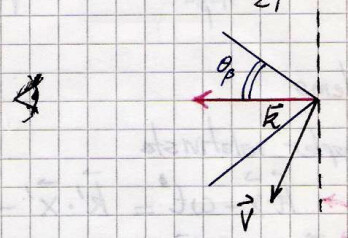
\includegraphics[width=0.3\textwidth]{images/fig_ft1_sr_dopplerA.jpg}

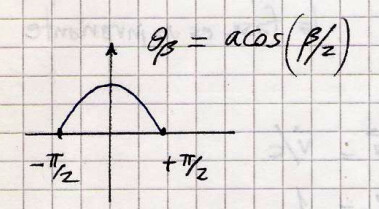
\includegraphics[width=0.3\textwidth]{images/fig_ft1_sr_dopplerB.jpg} 
 
\end{ejemplo}

\begin{ejemplo}{\bf Problema}

\[
	\tan\theta' = \gamma \sin\theta /( \cos\theta - \beta)
\]
y basta con ver lo que sucede en $\theta'= \pi/2, -\pi/2$. En su mayor parte, la energía toda
se va para adelante.

\end{ejemplo}


\subsection{Transcurso del tiempo en un sistema con V grande}

Sea $v/c$ no despreciable 
\[
	c \Delta t' = \gamma ( c\Delta t - \beta \Delta z) \qquad \qquad \gamma >1
\]
\[
	\Delta t' = \gamma \Delta t \left( 1 - \beta \frac{\Delta z}{c\Delta t} \right)
\]
pero si en $S'$ la partícula está en reposo es $v = dz/dt $ de manera que 
\begin{figure}[htb]
	\begin{center}
	\includegraphics[width=0.3\textwidth]{images/fig_ft1_vgrande.pdf} 
	\end{center}
	\caption{}
\end{figure} 
\[
	\Delta t' = \gamma \Delta t ( 1 - \beta^2)
\]
\[
	\Delta t' = \Delta t ( 1 - \beta^2)^{1/2}
\]
de modo que $ \Delta t' < \Delta t$, en $S'$ el tiempo transcurre más lentamente.

\subsubsection{Número de onda y conteo}

Un proceso de conteo (discreto) es invariante lorentziano, pero no así el medir
longitudes.
Supongamos un aparato que cuenta el número de crestas de ondas (que viajan con velocidad
$c$).
Cuento en $x^3$ entre

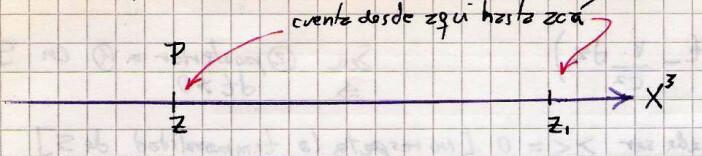
\includegraphics[width=0.6\textwidth]{images/fig_ft1_sr_ondas.jpg}

\[
	x'^3 = \gamma ( x^3 - \beta x^0 )
\]
siendo \vb{v} entre los sistemas $S$ y $S'$.
El número de crestas que cuenta el aparato es 
\[
	\#_s = \frac{ z_1 - z }{ \lambda } = \frac{ k }{ 2\pi }( z_1 - z ) = \frac{ k }{ 2\pi }( ct - z ) = 
	\frac{ 1 }{ 2\pi }( \omega t - kz )
\]
donde se ha usado que $z_1 = ct $, luego para un observador primado se tendrá consecuentemente
\[
	\#_s' = \frac{ 1 }{ 2\pi }( \omega' t' - k'z' )
\]
y se puede generalizar
\[
	\pe{k'}{x'} - \omega' t' = \pe{k}{x} - \omega t,
\]
lo cual nos conduce a ver que
\[
	-\left( \pe{k'}{x'} - \frac{\omega' x'^0 }{c} \right) = 
	-\left( \pe{k}{x} - \frac{\omega x^0 }{c}  \right)
\]
es un invariante lorentziano de acuerdo con
\be
	k_\alpha x^\alpha = k_{\alpha}' x^{'\alpha}
	\label{escalar_kx}
\ee
Entonces dado ese comportamiento se puede definir el cuadrivector de onda como
\[
	k^\alpha = \left( \frac{\omega}{c}, \vb{k}\right).
\]

Una onda plana debe ser invariante relativista. En una onda plana la ecuación de invariancia
\eqref{escalar_kx} conduce al efecto Doppler. En el caso relativista depende de la velocidad
relativa entre fuente y observador.

\subsection{Efecto Doppler relativista}

Volamos a la transformación entre sistemas $S$ y $S'$, teníamos
\[
	k'_z = \gamma \left( k_z - \beta \frac{\omega}{c} \right) \qquad \qquad 
	\frac{\omega'}{c}  = \gamma \left( \frac{\omega}{c} - \beta k_z \right)
\]
y de estas dos diferentes $k_z$ surge el efecto Doppler.
Se tienen los sistemas (el sin primar es en una galaxia)

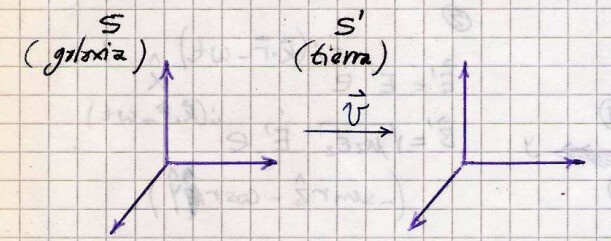
\includegraphics[width=0.6\textwidth]{images/fig_ft1_sperel_doppler1.jpg}

y serán
\[
	k_z = k \cos\theta \qquad 
	\frac{\omega'}{\gamma \omega} = 1 - \beta \cos \theta
\]
donde $\theta$ es el ángulo del número de onda con el eje $\zver$.
Considerando la transformación inversa (acercamiento)
$ \omega  = \omega' \gamma \left( 1 + \beta \cos\theta' \right) $ resulta
\[
	\frac{\omega'}{\gamma \omega} = \frac{ 1 }{ \gamma^2( 1 + \beta \cos \theta' ) }
\]

Ahora bien, tomando $\beta \ll 1 $ resulta
\[
	\omega \approx \omega \left( 1 - \frac{v}{c} \cos\theta \right)
\]
y a primer orden, con $\theta \sim \theta'$ usando 
\[
	\tan\theta = \frac{\sin\theta}{\gamma(\cos\theta -\beta)}.
\]

Veamos casos particulares de la invariancia del producto escalar.

{\bf Caso 1}

En este caso son paralelos la velocidad y el vector de onda, i.e. $\vb{v} \parallel \vb{k}$
se tienen $k_x=k_y=0$ y $k_z=k$ entonces
\[
	k' =  \gamma k (1 - \beta) = k \sqrt{ \frac{1-\beta}{1+\beta} }
\]
luego,
\[
	\omega' = \omega \sqrt{ \frac{1-\beta}{1+\beta} } \qquad 
	\lambda' = \lambda \sqrt{ \frac{1+\beta}{1-\beta} }
\]
donde $\beta > 0 $ implica alejamiento y $\beta < 0 $ implica acercamiento.
Luego la diferencia de longitudes de onda es
\[
	\Delta \lambda = \lambda' - \lambda = 
	\lambda \: \frac{ \sqrt{1+\beta} - \sqrt{1-\beta} }{ \sqrt{1-\beta} } 
	\approx \lambda \beta
\]
de lo cual se deduce que a primer orden en $\beta$ es $\Delta\lambda \sim \lambda\beta$.

Queríamos ver si es una buena aproximación, usamos
\[
	\frac{\lambda'}{\lambda} = \sqrt{\frac{1+\beta}{1-\beta}} = 
	\frac{ 14580 \:\mathrm{ \AA} }{ 6560 \:\mathrm{ \AA}}
\]
que es el cociente entre la longitud de onda medida en la tierra respecto de la misma
que viene de la estrella.
Entonces
\[
	\Frac{\lambda'}{\lambda}^2 = \Frac{1+\beta}{1-\beta}^{-1} = 0.202
\]
de modo que $\beta = 0.664$. Pero usando la aproximación
\[
	\beta = \frac{\Delta \lambda}{\lambda} = 1.223.
\]
Y entonces es claro que se necesita $\beta$ chico para que valga la aproximación hecha
más arriba.

{\bf Caso 2}

En este caso son perpendiculares la velocidad y el vector de onda, i.e. $\vb{v} \perp \vb{k}$,
se tiene un efecto Doppler transversal.

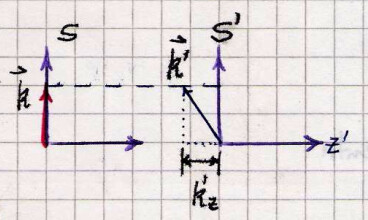
\includegraphics[width=0.3\textwidth]{images/fig_ft1_sperel_doppler2.jpg}

Se tienen en este caso $k_x' = k_x,  k_y'= k_y , k_z = 0 $ y es
\[
	k_z'= - \gamma \beta k  \qquad 
	{k'}^2= \gamma^2 k^2
\]
de modo que $ k' = \gamma k $ y $ \omega' = \gamma \omega $.
Vemos que en este caso el efecto Doppler transversal es notable solo a orden dos, es un fenómeno
netamente relativista ($\gamma$ es de orden cuadrado en su efecto). A orden cero (clásico) no hay
efecto.

Supongamos una partícula a velocidad constante según el observador $S$. Sean dos sucesos de esa
partícula.
\[
	c \Delta t' =  \gamma c \Delta t \left( 1 - \frac{\beta}{c} \frac{\Delta z}{\Delta t} \right)
\]
\[
	\Delta t' = \Delta t \sqrt{1 - \beta^2} = \frac{\Delta t}{\gamma}
\]
donde el intervalo de tiempo primado es tiempo propio pues en $S'$ la partícula está en reposo.
Se ve que en el sistema $S'$ el tiempo transcurre más lentamente, $ \Delta t' < \Delta t $.

Si no hay sistema en el cual se halle en reposo, podemos pensar en un intervalo infinitesimal
donde está en reposo instante a instante pero cambia.
\[
	dt'=  \sqrt{ 1 - \beta^2 } dt = d\tau
\]

\subsubsection{Ejemplo relojes}

Tenemos la situación depicted en el figurin:

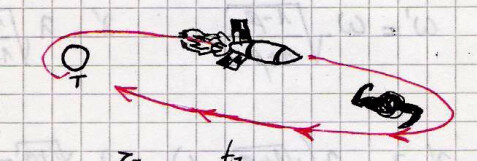
\includegraphics[width=0.6\textwidth]{images/fig_ft1_sperel_mellizos.jpg}

Tenemos un reloj 1 en S y un reloj 2 en S' dando la vuelta a la galaxia.
Se tiene
\[
	\tau_2 - \tau_1 = \int_{\tau_1}^{\tau_2} d\tau = 
	\int_{t_1}^{t_2} \sqrt{ 1 - \frac{v^2(t')}{c^2}} dt < t_2 - t_1
\]
y estos sistemas no son equivalentes. Es la paradoja de los mellizos.
El tiempo pasa más lento para el que viajó
\[
	\tau_2 - \tau_1 = \frac{1}{c} \int_{a}^{b} ds
\]

La métrica de Minkowski no corresponde a una euclideana.

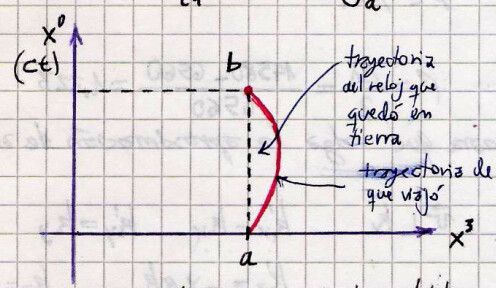
\includegraphics[width=0.6\textwidth]{images/fig_ft1_sperel_mellizos2.jpg}

En el espacio de Minkwoski la línea recta es la distancia mayor entre dos puntos.


% =================================================================================================
\section{Forma covariante del electromagnetismo}
% =================================================================================================

Partimos de la ecuación de continuidad para la carga,
\[
	\dpar{\rho}{t} + \divem{J} = 0
\]
\notamargen{La conservación de la carga es una de las leyes más firmemente establecidas.}
la cual con la definición del cuadrivector corriente
\[
	J^\mu = ( c\rho , \vb{J} )
\]
se puede escribir como 
\[
	\partial_\mu J^\mu = \dpar{ (c\rho)}{(ct)} + \divem{J} = 0 .
\]

La formulación covariante empleaba el gauge de Lorentz (es necesario) puesto que con él las 
ecuaciones son válidas en cualquier sistema inercial. El gauge de Lorentz era
\[
	\frac{1}{c} \dpar{\phi}{t} + \divem{A} = 0
\]
siendo el cuadripotencial
\[
	A^\mu = ( \phi , \vb{A} ) 
\]
y entonces 
\[
	\partial_\mu A^\mu = \dpar{\phi}{ct} + \divem{A} = \frac{1}{c} \dpar{\phi}{t} + \divem{A} = 0 .
\]

Se podía ver que resultan ecuaciones de onda inhomogéneas para los potenciales
\[
	\Nabla^2 \vb{A} - \frac{1}{c^2} \dpar[2]{\vb{A}}{t} = -\frac{4\pi}{c} \vb{J}
\]
que viene a ser, usando el D'alembertiano, 
\[
	\partial_\mu\partial^\mu = \Box \vb{A} = \frac{4\pi}{c} \vb{J}
\]
y para el potencial $\phi$
\[
	\Nabla^2 \phi - \frac{1}{c^2} \dpar[2]{\phi}{t} = - 4\pi \phi
\]
que desemboca en 
\[
	\partial_\mu\partial^\mu = \Box \phi = \frac{4\pi}{c} ( c\rho )
\]

Al aplicar el D'Alembertiano a un cuadrivector obtenemos otro cuadrivector 
\[
	\Box A^\mu = \frac{4\pi}{c} J^\mu.
\]


Veamos qué sucede con las ecuaciones de Maxwell en forma tensorial.
Recordemos que toda ecuación de igualdad de entes tensoriales en el espacio
de Minkowski es covariante.
\notamargen{Otros gauges sirven bien si no me interesa pasar de un sistema a otro.}

Teníamos
\[
	\vb{E} = -\Nabla \phi - \frac{1}{c}\dpar{\vb{A}}{t}, 
\]
de modo que en términos del cuadripotencial
\[
	E_i = - \partial_i A^0 -\partial^0 A^i = -( \partial^0 A^i - \partial^i A^0)
\]
y luego el campo $\vb{B}$ viene del rotor del cuadripotencial, por lo tanto
\[
	B_x = \dpar{A_z}{y} - \dpar{A_y}{z} = \partial^3A^2 - \partial^2A^3
\]
del mismo modo que
\[
	B_y = \dpar{A_x}{z} - \dpar{A_z}{x} = \partial^1A^3 - \partial^3A^1 \qquad 
	B_z = \partial^2A^1 - \partial^1A^2
\]
y entonces se puede definir un ente
\[
	F^{\alpha\beta} = \partial^\alpha A^\beta - \partial^\beta A^\alpha
\]
que unifica notaciones para los dos campos.

Los campos \vb{E}, \vb{B} forman parte de un tensor de segundo rango antisimétrico llamado tensor
de intensidad de campo (tiene diagonal nula),
\[
	F^{\alpha\beta} = \partial^\alpha A^\beta - \partial^\beta A^\alpha
\]
que tendrá seis elementos independientes. Tres para el campo eléctrico y tres para el magnético.
Matricialmente se puede ver como 
\[
	F^{\alpha\beta} =
	\begin{pmatrix}
	 0 & -E_x & -E_y & -E_z \\
	 E_x & 0 & -B_z & B_y \\
	 E_y & B_z & 0 & -B_x \\
	 E_z & -B_y & B_x & 0 \\
	\end{pmatrix}
\]
Utilizando la métrica $g_{\mu\nu}$ podemos arribar a la versión covariante
\[
	F_{\alpha\beta} = g_{{\alpha\mu}} g_{{\alpha\nu}} F^{\mu\nu} 
	= g_{{\alpha\mu}} F^{\mu}_{\ \alpha}
\]
\[
	F_{\alpha\beta} =
	\begin{pmatrix}
	 0 & E_x & E_y & E_z \\
	 E_x & 0 & -B_z & B_y \\
	 E_y & B_z & 0 & B_x \\
	 E_z & -B_y & B_x & 0 \\
	\end{pmatrix}
\]

También es conveniente definir un tensor de intensidad de campo dual,
con ambos índices contravariantes,
\[
	\mathcal{F}^{\alpha\beta} =  \frac{1}{2} 
	\vare^{\alpha\beta\gamma\delta} F_{\gamma\delta}
\]
que no es otra cosa que 
\[
	\mathcal{F}^{\alpha\beta}=
	\begin{pmatrix}
	 0 & -B_x & -B_y & -B_z \\
	 B_x & 0 & E_z & -E_y \\
	 B_y & -E_z & 0 & E_x \\
	 B_z & E_y & -E_x & 0 \\
	\end{pmatrix}
\]
y donde $\varepsilon^{\alpha\beta\gamma\delta}$ es el tensor de Levi-Civita 
de cuatro dimensiones -totalmente antisimétrico-, que es nulo cuando se repite un índice.

\begin{ejemplo}{\bf Tensor dual}

Sea por ejemplo el elemento $\mathcal{F}^{01}$,
\[
	\mathcal{F}^{01} = \frac{1}{2} \: \vare^{01\gamma\delta} \: F_{\gamma\delta},
\]
así que dado el comportamiento del tensor de Levi-Civita se tienen
\[
	\mathcal{F}^{01} = \frac{1}{2} \: \left( 
	\vare^{ 0123} \: F_{23} +
	\vare^{ 0132} \: F_{32}
	\right),
\]
dado que toda otra posibilidad es nula. Entonces
\[
	\mathcal{F}^{01} = \vare^{ 0123}  \: F_{23}
\]
y vemos que se pasa del $F$ al $\mathcal{F}$ con la regla
\[
	\vb{E}\to\vb{B} \qquad \qquad \vb{B}\to -\vb{E}
\]
\end{ejemplo}


Se querrá entonces escribir las ecuaciones de Maxwell en forma covariante explícita, lo
que significa que no cambiarán de forma al pasar entre sistemas inerciales.

Tomamos las dos ecuaciones con fuentes, y se ve que las podemos expresar según
\[
	\partial_i E_i = \frac{4 \pi }{c} J^0 = \partial_i F^{i0} = \partial_{\alpha} F^{\alpha 0},
\]
asimismo
\[
	\partial_2 B_{3} - \partial_3 B^{2} - \partial_0 E^{1} = 
	\frac{4 \pi }{c} J^1 = \partial_{\alpha} F^{\alpha 1}
\]
es la componente 1 del mismocuadrivector. Entonces
\[
	\partial_\alpha F^{\alpha\beta} =  \frac{4 \pi}{c} J^\alpha.
\]
resume las dos ecuaciones de Maxwell con fuentes.

Con respecto a las ecuaciones sin fuentes
\[
	\partial_i \mathcal{F}^{0i} =  0 =
	\partial_\alpha \mathcal{F}^{0\alpha} 
\]
entonces 
\[
	\partial_\alpha \mathcal{F}^{\alpha \beta}  = 0
\]
resume las ecuaciones sin fuentes.
Si se usa el tensor directo quedan expresadas como
\[
	\partial^\alpha \mathcal{F}^{\beta\gamma} +
	\partial^\beta \mathcal{F}^{\gamma\alpha} +
	\partial^\gamma \mathcal{F}^{\alpha\beta} = 0.
\]
Recordemos que usaremos índices griegos para los cuatros componentes $0,1,2,3$ e índices
latinos para la parte espacial $1,2,3$.

\begin{ejemplo}{\bf Comentario corrientes parásitas}

Un conductor en el seno de un campo magnético genera sobre sí al moverse corrientes
de Foucault o turbillonarias que tienden a frenar su movimiento.
 
\end{ejemplo}


\subsection{Transformación de los campos}

Volviendo a la transformación de Lorentz de los sistemas $S$ a $ S'$ 
\begin{align*}
	ct' &= \gamma \: [ ct - \pe{\beta}{x} ] \\
	\mathbf{x'}_\parallel &= \gamma \: [ \mathbf{x}_\parallel - {\beta}ct ] \\
	\mathbf{x'}_\perp &= \mathbf{x}_\perp
\end{align*}
con $\vb{\beta} = \vb{v}/c$ y siendo la matriz de la transformación la siguiente
\[
	a^{\mu}_{\nu} = 
	\begin{pmatrix}
	\gamma & 0 & 0 & -\gamma\beta \\
	0 & 1 & 0 & 0 \\
	0 & 0 & 1 & 0 \\
	-\gamma\beta & 0 & 0 & \gamma
	\end{pmatrix}
\]
se tiene $ F^{\mu\nu'} = a^{\mu}_{\lambda} a^{\nu}_{\sigma} F^{\lambda\sigma}$
donde $ F^{\lambda\sigma} $ es el tensor con índices contravariantes.

\begin{figure}[htb]
	\begin{center}
	\includegraphics[width=0.4\textwidth]{images/fig_ft1_transfCampo1.pdf}
	\includegraphics[width=0.4\textwidth]{images/fig_ft1_transfCampo2.pdf} 
	\end{center}
	\caption{}
\end{figure} 

La transformación de los campos \vb{E}, \vb{B} según la figura superior satisface 
\begin{align*}
	&E'_x = \gamma ( E_x - \beta B_y ) &\qquad B'_x = \gamma ( B_x + \beta E_y ) \\
	&E'_y = \gamma ( E_y + \beta B_x ) &\qquad B'_y = \gamma ( B_y - \beta E_x ) \\
	&E'_z = E_z \qquad \qquad \qquad & \qquad \qquad \qquad B'_z = B_z &  
\end{align*}
y separando los campos en componentes paralelas y perpendiculares, esto es
$\vb{E} = \vb{E}_\parallel + \vb{E}_\perp $ y $\vb{B} = \vb{B}_\parallel + \vb{B}_\perp $
se tienen
\[
	\vb{E}' = \vb{E}_\parallel + \gamma \: ( \vb{E}_\perp  + \pv{\beta}{B} )
\]
\[
	\vb{B}' = \vb{B}_\parallel + \gamma \: ( \vb{B}_\perp  - \pv{\beta}{E} )
\]
que se pueden poner como 
\[
	\vb{E}' = - \frac{ \gamma^2 }{ \gamma + 1 }\vb{\beta} (\pe{\beta}{E}) +
		\gamma \: ( \vb{E}  + \pv{\beta}{B} )
\]
\[
	\vb{B}' = - \frac{ \gamma^2 }{ \gamma + 1 }\vb{\beta} (\pe{\beta}{B}) + 
		\gamma \: ( \vb{B}  - \pv{\beta}{E} ).
\]

Recordemos que la transformación de Galileo era
\[
	\vb{E}' = \vb{E} + \frac{1}{c} \pv{V}{B} \qquad \qquad 
	\vb{B}' = \vb{B} - \frac{1}{c} \pv{V}{E}
\]
siendo el segundo término el que da origen a las corrientes de Foucault al mover 
un conductor en el seno de un campo \vb{B}.
Las chapas en un transformador aisladas buscan cortas las corrientes de Foucault.
No conviene diseñar un aparato que tenga que moverse en el seno de un campo
magnético si es de material conductor.


Las contracciones del producto escalar entre el tensor de intensidad son invariantes.
\notamargen{Como estamos poniendo contracciones opuestas se compensan los efectos 
entre sí y dan invariantes [?].}
Así, por ejemplo,
\begin{align*}
	F^{\alpha\beta}F_{\alpha\beta} &= 2( B^2 - E^2 ) \\
	\mathcal{F}^{\alpha\beta}\mathcal{F}_{\alpha\beta} &= 2( E^2 - B^2 ) \\
	\mathcal{F}^{\alpha\beta}F_{\alpha\beta} &= -4 \: \pe{B}{E}
\end{align*}

Sea 
\[
	\mathcal{F}^{\alpha\beta}F_{\alpha\beta} = -4 \: \pe{B}{E} = 0,
\]
entonces $\vb{E} \perp \vb{B}$ o alguno de los campos es nulo en todo sistema inercial.
Lo mismo si se tiene que el invariante es mayor a cero; lo será en todos los sistemas
inerciales.

Para una carga que se mueve con velocidad \vb{v} se tiene $\vb{B}=0$ en un sistema en 
el que $q$ está en reposo de manera que 
\[
	\pe{B}{E} = \pe{B'}{E'} = 0
\]
siempre y entonces $\vb{E'} \perp \vb{B'}$ para cualquier sistema inercial $S'$. El 
campo magnético que crea la partícula será perpendicular al campo eléctrico en toda
situación.

Un sistema electromagnético dependiente del tiempo intercambiará \vb{p} con el campo entonces no vale el
principio de acción y reacción ,
\[
	\dtot{\vb{P}_M}{t} + \dtot{\vb{P}_c}{t} = \int_{S(v)} \overline{T}\cdot d\vb{S}
\]
mientras que 
\[
	\dtot{\vb{P}_c}{t} = \dtot{}{t} \left( \frac{1}{4\pi c} \int \pv{E}{B} dV \right)
\]

\subsection{Covarianza con medios materiales}

Las ecuaciones sin fuentes tienen la misma forma en presencia de medios materiales.
Las que cambian son las que tienen fuentes, porque ahora aparecen los campos $\vb{H}$
y $\vb{D}$.

Para un medio material podemos reemplazar el tensor $F^{\alpha\beta} $ por otro
tensor $ G^{\alpha\beta}  $ tal que 
\[
	E_i \to D_i, \qquad B_i \to H_i
\]
donde 
\[
	G^{\alpha\beta} =
	\begin{pmatrix}
	 0 & -D_x & -D_y & -D_z \\
	 D_x & 0 & -H_z & H_y \\
	 D_y & H_z & 0 & -H_x \\
	 D_z & -H_y & H_x & 0 \\
	\end{pmatrix}
\]
que se puede pensar como otro tensor corrector?
\[
	F^{\alpha\beta} = G^{\alpha\beta} + R^{\alpha\beta}, 
\]
donde 
\[
	R^{\alpha\beta} = 4 \pi
	\begin{pmatrix}
	 0 & -P_x & -P_y & -P_z \\
	 P_x & 0 & M_z & -M_y \\
	 P_y & -M_z & 0 & M_x \\
	 P_z & -M_y & M_x & 0 \\
	\end{pmatrix}
\]
que provienen de las relaciones constitutivas
\[
	\vb{D} = \vb{E} + 4\pi\vb{P} \qquad\qquad \vb{H} = \vb{B} - 4\pi\vb{M}.
\]
Finalmente
\[
	\partial_\alpha G^{\alpha\beta} = \frac{4\pi}{c} J^\beta
\]
donde la información de $P_i$ y $M_i$ está en el tensor $R^{\alpha\beta}$.
Estamos diciendo que en un medio material los vectores $\vb{P}, \vb{M}$ se deben
comportar como los elementos de un tensor.

Procediendo en forma análoga a lo que se hiciera para los campos $\vb{E}$ y $\vb{B}$
en la transformación de Lorentz, se tendrán los campos transforman según 
\[
	\vb{P}' = \vb{P}_\parallel + \gamma \: ( \vb{P}_\perp  - \pv{\beta}{M} )
\]
\[
	\vb{M}' = \vb{M}_\parallel + \gamma \: ( \vb{M}_\perp  + \pv{\beta}{P} )
\]

Entonces de un sistema inercial a otro una \vb{P} da origen a una \vb{M} y viceversa.

% =================================================================================================
\section{Principio de Hamilton y relatividad}
% =================================================================================================

Habiéndonos situado en un espacio de Minkowski, tenemos la acción
\[
	S = -\alpha \int_a^b ds,
\]
siendo $\alpha$ una constante a fijar luego, y $ds$ un arco en el espacio minkowskiano entre
dos eventos $a$ y $b$. 
La acción debe ser un invariante pues es un extremo y el intervalo $ds$ debe ser temporal,
\[
	ds = \sqrt{ c^2 dt^2 - dx^2 - dy^2 - dz^2 } = 
	c \: \sqrt{ 1 - v^2/c^2 } \: dt
\]
de manera que 
\[
	S = -\alpha \int_{t_1}^{t_2} c \sqrt{ 1 - v^2/c^2 } \: dt = 
	\int_{t_1}^{t_2} \mathcal{L} dt
\]
y donde $\mathcal{L}$ es el lagrangiano, 
\[
	\mathcal{L} = -\alpha c \left( 1 - v^2/c^2 \right)^{1/2} \approx -\alpha c + \frac{\alpha v^2}{2c}
\]
y luego 
\[
	\mathcal{L} \to T = \frac{m v^2}{2} \; \text{(baja velocidad)}
\]
de manera que fijamos el valor de la constante a partir de este límite de baja velocidades,
\[
	\mathcal{L} = -m c^2 \left( 1 - v^2/c^2 \right)^{1/2}
\]
es el lagrangiano relativista.

A partir de las ecuaciones de Euler-Lagrange es 
\[
	p_i = \dpar{\mathcal{L}}{\dot{q}_i} = \dpar{\mathcal{L}}{v_i}
\]
y haciendo el álgebra,
\[
	p_i = \frac{ m v_i }{\sqrt{ 1 - v^2/c^2 }},
\]
donde $m$ es la masa en reposo y $p_i$ es el momento relativista. 
Notemos que si $v=c$ entonces el momento diverge si $m\neq 0$, mientras que con m=0 no sabemos
qué sucede.
Entonces
\[
	\dtot{\vb{P}}{t} = m \dtot{}{t}\left( \frac{\vb{v}}{\sqrt{1 - v^2/c^2 }}\right).
\]

Para un movimiento circular, el módulo de la velocidad permanece constante.
\[
	\dtot{|\vb{v}|}{t} = 0 \quad \Rightarrow \quad \dtot{\vb{P}}{t} =
		\left( \frac{ m }{\sqrt{1 - v^2/c^2 }}\right) \dtot{\vb{v}}{t} =
		m \: \gamma \: \dtot{\vb{v}}{t}
\]
si en cambio es $ \dtot{|\vb{v}|}{t} \neq 0 $ se tiene 
\[
	\dtot{\vb{P}}{t} = m \left( \left( \frac{ 1 }{\sqrt{1 - v^2/c^2 }}\right) \dtot{\vb{v}}{t} 
	+ \vb{V} (1 - v^2/c^2)^{-3/2} \frac{v}{c^2} \dtot{v}{t} \right)
\]
\[
	\dtot{\vb{P}}{t} = m \gamma \dtot{\vb{v}}{t} + m \vb{v} \gamma^3 \frac{v}{c^2} \dtot{v}{t}
\]
donde el primer término en el RHS está asociado a la variación en la dirección y el segundo a la variación
en la magnitud (hemos usado con $ \gamma^3 v^2/c^2 > \gamma $ ?). De esto se desprende que la inercia es
mayor para variar la longitud de \vb{v} que su dirección. Es más fácil cambiar dirección que rapidez.
\notamargen{En la carpeta hay otra cosa: Tengo
$ \dtot{\vb{p}}{t} = \gamma^3 m \dtot{\vb{v}}{t} $.}

Entonces, volviendo al langrangiano
\[
	E = \pe{p}{v} - \Lag = m \gamma v^2 + m c^2 \gamma^{-1} = m \gamma c^2
\]
y esta es la energía relativista de una partícula libre. 
\notamargen{Anoté que esta energía es compatible con el PAM,
que calculo será el principio de acción mínima.}
Veamos el límite de bajas velocidades, es decir
que si $v/c \ll 1$ entonces 
\[
	\gamma = \sqrt{ 1 - v^2/c^2 } \approx 1 + \frac{v^2}{2c^2},
\]
y resulta 
\[
	E \approx  m c^2 + \frac{m v^2}{2} = E_0 + \frac{m v^2}{2}
\]
donde $E_0$ es una energía en reposo, que no depende de \vb{v} y podemos 
expresar la energía cinética como 
\[
	E - m c^2 = \frac{m v^2}{2} = T.
\]

Se puede definir
\[
	\vb{p} = m \vb{w},
\]
con $\vb{w} = \gamma \vb{v}$ entonces 
\[
	E^2 = m^2 \gamma^2 c^4 \qquad p^2 = m^2 \gamma^2 v^2 
\]
y
\[
	\frac{E^2}{c^2} = m^2 c^2 \gamma^2
\]
\[
	\frac{E^2}{c^2} - p^2 = m^2 \gamma^2 (c^2 -v^2) = m^2 c^2
\]
y esta es la relación fundamental entre energía y momento 
\[
	\frac{E^2}{c^2} = p^2 + m^2c^2.
\]

Para partículas con $m_0 = 0$ y $v=c$ será 
\[
	\frac{E^2}{c^2} = p^2 \qquad \qquad p = \frac{h\nu}{c} = k\hbar.
\]

La formulación hamiltoniana comenzará a partir de 
\[
	\Ham = \sqrt{ p^2 + m^2 c^2} \: c,
\]
sobre el que se puede operar para obtener el límite clásico (de bajas velocidades) como 
\[
	\Ham = \left( 1 + \frac{ p^2 }{ m^2 c^2 } \right)^{1/2} m c^2
\]
y si se cumple $ p/(mc) \ll 1$ entonces 
\[
	\Ham \approx mc^2 + \frac{ p^2 }{2m^2}
\]
donde el último término  es el hamiltoniano de la mecánica clásica para nuestra partícula
libre.

El cuadrimomento se define como 
\[
	p^\mu = ( m\Gamma c , m \Gamma \vb {u}), \qquad \Gamma \equiv \frac{ 1 }{ \sqrt{ 1 - v^2/c^2 } } 
\]
o bien 
\[
	p^\mu = ( E/c , \vb{p} )
\]
siendo 
\[
	p^\mu p_\mu = \frac{E^2}{c^2} - p^2 = m^2 c^2
\]
el invariante asociado a la conservación (del cuadrimomento).

\begin{ejemplo}{\bf Problema 11}
 
Se espera que al tener una carga en movimiento aparezca en alguna parte una corriente.
Consideramos un sistema $K'$ en movimiento relativo con respecto a otro sistema $K$.
Con las definiciones usuales de $\beta$ y $\gamma$ tendremos
\[
	\vb{E}_\parallel' = \vb{E}_\parallel \qquad \qquad  
	\vb{E}_\perp' = \gamma ( \vb{E}_\perp + \pv{\beta}{B} )
\]
\[
	\vb{B}_\parallel' = \vb{B}_\parallel \qquad \qquad  
	\vb{B}_\perp' = \gamma ( \vb{B}_\perp - \pv{\beta}{E} )
\]
de lo cual las inversas
\[
	\vb{E}_\perp' = \gamma ( \vb{E}_\perp - \pv{\beta}{B}' ) \qquad \qquad 
	\vb{B}_\perp' = \gamma ( \vb{B}_\perp' + \pv{\beta}{E}' )
\]

Introduciendo la física en la transformación
\[
	\vb{E}' = q \: \frac{\vb{x}'}{|\vbx'|^3} \qquad \qquad \vb{B}' = 0
\]
y tendríamos que convertir a coordenadas sin primar.
\[
	\vb{E}_\parallel = \vb{E}_\parallel' =  q \: \frac{\vb{x}_\parallel'}{|\vbx'|^3} 
	\qquad \qquad  \vb{E}_\perp = \gamma \vb{E}_\perp' 
\]
\[
	\vb{B}_\parallel = \vb{B}_\parallel' = 0 \qquad \qquad  
	\vb{B}_\perp = \gamma \pv{\beta}{E}_\perp' 
\] 
donde son
\[
	\vbx_\parallel' = \gamma ( \vbx_\parallel - c \vb{\beta}t ) 
	\qquad \qquad \vbx_\perp' = \vbx_\perp,
\]
y luego la norma será
\[
	|\vbx'|^2 = |\vbx_\parallel'|^2 + |\vbx_\perp'|^2 =
	\gamma^2 ( \vbx_\parallel - c \vb{\beta}t )^2 + |\vbx_\perp'|^2
\]
Juntando todo podemos escribir
\[
	\vb{E}_\parallel = \frac{q ( \vbx_\parallel - c \vb{\beta}t ) }
	{ (\gamma^2 ( \vbx_\parallel - c \vb{\beta}t )^2 + |\vbx_\perp'|^2)^{3/2} } 
	\qquad \qquad  
	\vb{E}_\perp = \frac{ q \: \gamma \vbx_\perp }
	{ (\gamma^2 ( \vbx_\parallel - c \vb{\beta}t )^2 + |\vbx_\perp'|^2)^{3/2} } 
\]
\[
	\vb{B}_\parallel = 0 \qquad \qquad  
	\vb{B}_\perp = \pv{\beta}{E}_\perp 
\] 
Entonces tenemos dos partículas con velocidad perpendicular.
Un sistema dependiente del tiempo intercambia momento con el campo.
 
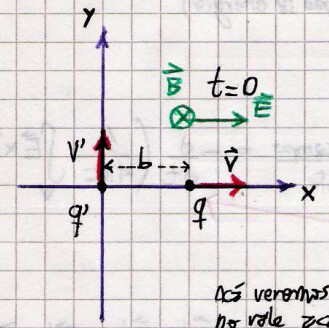
\includegraphics[width=0.4\textwidth]{images/fig_ft1_speRel_prob11A.jpg} 
 
Aquí tenemos la expresión de los campos producidos por una partícula en movimiento vista
desde un sistema reposante, el sistema que se mueve está en la partícula.
Presupusimos que ambos coinciden en $x=0$ y $t=0$.
En esta situación se verá que no vale acción y reacción.

Veamos ahora los campos para $q'$ donde 
\[
	\vb{\beta}' = \frac{V'}{c}\yver \qquad \qquad \gamma' = \frac{1}{\sqrt{ 1 - {\beta'}^2}}
\]
\[
	\vb{E}_\parallel = 0 (t=0)  \qquad \qquad  
	\vb{E}_\perp = \gamma' q' \frac{1}{b} \xver 
\]
\[
	\vb{B}_\parallel = B_y \yver = 0 \qquad \qquad  
	\vb{B}_\perp = - \frac{\gamma' q' V' }{cb^2} \zver 
\]  
y la fuerza de Lorentz, sobre $q$ debido a $q'$, será
\[
	\vb{F} = \frac{\gamma q q'}{b^2}\left( \xver + \frac{VV'}{c^2} \yver \right)
\]
 
Ahora corremos el sistema de referencia, que es el eje $\yver$. Recordemos que los sistemas
siempre están en reposo. No están en movimiento relativo.

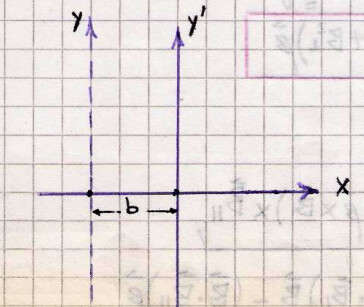
\includegraphics[width=0.4\textwidth]{images/fig_ft1_speRel_prob11B.jpg} 

Se tienen ahora
\[
	\vb{E}_\parallel = - \frac{ q }{ \gamma^3 b^2} \xver \qquad \vb{E}_\perp = 0 
	\vb{B}_\parallel = 0 \qquad \qquad  \vb{B}_\perp = 0
\]
de tal manera que el campo total es $\vb{B}=0$ y $\vb{E}=\vb{E}_\parallel$.
La fuerza será
\[
	\vb{F} = - \frac{q q'}{\gamma^3 b^2} \xver ,
\]
y vemos que no es la misma expresión.

Hay momento que se va hacia alguna parte; las partículas transfieren momento hacia afuera
(hacia el campo).
\[
	\vb{P}_\text{campo} = \frac{1}{4\pi} \int_V \: \pv{E}{B} \: dV
\]
pero habría que calcular el campo para todo el espacio puesto que el integrando abarca todo.
Si tomo el volumen muy grande y usamos la expresion [CITA]
\[
	\dtot{P_\text{mec}}{t} + \dtot{P_\text{campo}}{t}  = \int_{S(v)} T \cdot \nver dS,
\]
será la integral de surface nula pues no se escapa energía. Entonces
\[
	\dtot{P_\text{mec}}{t} = - \dtot{P_\text{campo}}{t}
\]
y la fuerza de Lorentz será
\[
	\vb{F}_\text{Lorentz} = - \dtot{P_\text{campo}}{t} = 
	-\dtot{}{t}\left( \frac{1}{4 \pi c} \int_V \: \pv{E}{B} \: dV \right)
\]
y esta cuenta debería dar lo mismo.
 
\end{ejemplo}

\begin{ejemplo}{\bf Problema 13}

Consideremos la cuenta
\[
	\pv{E'}{B'} = ( \vb{E}_\parallel' + \vb{E}_\perp' )\times( \vb{B}_\parallel' + \vb{B}_\perp' ) =
	\vb{E}_\parallel' \times \vb{B}_\parallel' +
	\vb{E}_\parallel' \times \vb{B}_\perp' +
	\vb{E}_\perp' \times \vb{E}_\parallel' +
	\vb{E}_\perp' \times \vb{B}_\perp' 
\]
que da cuatro términos de los cuales el primero es nulo, el segundo y tercero son proporcionales a
$\vb{\beta}_\perp$ mientras que el cuarto es proporcional a $\vb{\beta}_\parallel$.
Entonces tenemos la separación de los productos vectoriales de acuerdo con
\[
	( \pv{E'}{B'} )_\parallel = \pv{E'_\perp}{B'_\perp}
	\qquad \qquad 
	( \pv{E'}{B'} )_\perp = \pv{E'_\parallel}{B'_\perp} + \pv{E'_\perp}{B'_\parallel} 
\]
\[
	( \pv{E'}{B'} )_\parallel = \gamma^2 ( \vb{E}_\perp + \pv{\beta}{B} ) \times ( \vb{B}_\perp + \pv{\beta}{E} )
\]
\[
	( \pv{E'}{B'} )_\perp = \gamma \vb{E_\parallel} \times ( \vb{B}_\perp - \pv{\beta}{E} )
	+ \gamma ( \vb{E}_\perp + \pv{\beta}{B} ) \times \vb{B_\parallel} 
\]
que conducen a
\[
	\pv{E_\perp}{B_\perp} - ( \vb{E}_\perp \times \pv{\beta}{E} ) + ( \pv{\beta}{B} ) \times \vb{B_\perp}  - 
	( \pv{\beta}{B} ) \times ( \pv{\beta}{E} ) 
\]
de los cuales el primero es $(\pv{E}{B})_\parallel$, el segundo $-E^2_\perp \vb{\beta}$ mientras que
el tercero
\[
	(\pe{\beta}{B})\vb{\beta} - (\pe{B}{B_\perp})\vb{\beta} = - B^2_\perp \vb{\beta}
\]
y el cuarto
\[
	( (\pv{\beta}{E})\cdot \vb{B} ) \vb{\beta} - [ (\pv{\beta}{E})\cdot \vb{\beta} ]\vb{B} =
	[ (\pv{E}{B})\cdot \vb{\beta} ]\vb{\beta} = [ (\pv{E}{B})_\parallel \beta] \vb{\beta}
\]
de manera que 
\[
	(\pv{E'}{B'})_\parallel = \gamma^2 ( 1 + \beta^2 ) (\pv{E}{B})_\parallel -
	\gamma^2 ( E^2_\perp + B^2_\perp ) \vb{\beta}.
\]

Ahora operamos $ (\pv{E'}{B'})_\perp $ y obtenemos
\[
	\gamma (\pv{E}{B})_\perp - \gamma \vb{E}_\parallel \times (\pv{\beta}{E}) +
	\gamma ( \pv{\beta}{B}) \times \vb{B}_\parallel,
\]
y este último término se desarma como
\[
	\gamma (\pe{\beta}{B_\parallel})\vb{B} - (\pe{B}{B_\parallel})\vb{\beta} =
	(\pe{\beta}{B})\vb{B}_\perp
\]
y puede verse que sucede lo mismo con el término que contiene al campo $\vb{E}$ de modo que
\[
	(\pv{E'}{B'})_\perp = \gamma (\pv{E}{B})_\perp + \gamma (\pe{\beta}{E}) \vb{E}_\perp 
	+ \gamma (\pe{\beta}{B}) \vb{B}_\perp .
\]

Ahora habría que ver que hay un sistema de referencia donde se cumple que sean colineales.
Entonces el producto vectorial será nulo.
\[
	\begin{cases}
	( 1 + \beta^2 ) (\pv{E}{B})_\parallel = ( E^2_\perp + B^2_\perp ) \vb{\beta} \\
	(\pv{E}{B})_\perp = -(\pe{\beta}{E}) \vb{E}_\perp - (\pe{\beta}{B}) \vb{B}_\perp
	\end{cases}
\]
de manera que al ser colineales sucede que
\[
	( 1 + \beta^2 ) (\pv{E}{B}) = ( E^2_\perp + B^2_\perp ) \vb{\beta}  -
	( 1 + \beta^2 ) [ (\pe{\beta}{E}) \vb{E}_\perp + (\pe{\beta}{B}) \vb{B}_\perp ]
\]
y además
\[
	\frac{\vb{V}}{1 + V^2/c^2} = c \frac{\pv{E}{B}}{E^2+B^2}
\]
de tal modo que 
\[
	( E^2 + B^2 )\vb{\beta} = ( 1 + \beta^2 )( \pv{E}{B} )
\]
y se deduce que $ ( \pv{E}{B} )_\perp = 0 $.
Pero a la última parte no se llega fácil; presupongo $\pe{\beta}{E} = \pe{\beta}{B} = 0$
y entonces de $\pe{E}{B} = 0$ tenemos que ambos campos son perpendicularesy puede ser que
$\vb{E}= 0 = \vb{B}$, si en cambio son $\vb{E} \parallel \vb{B}$ (por lo que se vio antes) 
se tendrá $E^2 - B^2 < 0$ o bien $E^2 - B^2 > 0$; si en un sistema es $E=0$ entonces será
$B\neq 0$.
Estamos usando como invariantes $\pe{E}{B}$ y $E^2-B^2$.

\end{ejemplo}

\subsection{Principio de Hamilton e interacción electromagnética}

Se parte de una variación de la acción
\[
	\delta S = - m c \: \delta \int_a^b \: ds
\]
donde $ds = \sqrt{ g_{\alpha\beta}dx^\alpha dx^\beta}$ de manera que 
\[
	- m c \delta \int_a^b \: \sqrt{ g_{\alpha\beta}dx^\alpha dx^\beta} =
	- \frac{mc}{2} \int_a^b \: \frac{ \delta( dx_\mu dx^\mu)}{ \sqrt{ g_{\alpha\beta}dx^\alpha dx^\beta} }
	= - m \int_a^b \: \delta( dx_\mu ) \dtot{x^\mu}{\tau}
\]
donde nos hemos sacado la raíz de encima. Esto ahora se puede integrar por
partes,
\[
	\delta S = - m \int_a^b \: w^\nu \delta dx_\nu =  
	- m w^\nu dx_\nu |_a^b + m \int_a^b \: w_\nu \delta x^\nu
\]
y como $a$ y $b$ son puntos fijos, el primer término se anula. Luego
\[
	\delta S =  m \int_a^b \: w^\nu \delta (dx_\nu)
\]
o bien
\[
	\delta S =  m \int_a^b \: \dtot{w^\nu}{\tau} \delta x_\nu  d\tau =
	m \int_a^b \: a^\nu \delta x_\nu  d\tau,
\]
que implica que el cuadrivector aceleración $a^\mu$ debe ser nulo.
Luego, la cuadrivelocidad de la partícula debe ser constante.
Podemos escribir esta equivalencia 
\[
	\vb{p} = \Nabla S \quad \longrightarrow \quad  p^\mu = \partial^\mu S
\]

Consideremos ahora que el punto $a$ se varía (ya no es fijo) $ \delta x^\nu \equiv \delta x^\nu |_a \neq 0 $
de manera que 
\[
	\delta S = m w^\nu \delta x_\nu
\]
y
\[
	p^\nu = m w^\nu = \dpar{S}{x_\nu}
\]
entonces
\[
	w^\nu = (\gamma c, \gamma \vb{v})
\]
es proporcional a la energía de la partícula. Luego, $p^\nu = ( m \gamma c, m \gamma \vb{v})$ y
\[
	p^0 = m \gamma c = \frac{ m \gamma c^2 }{c} = \frac{E}{c} = \dpar{S}{x^0}
\]
de modo que
\[
	\partial_\mu  S \partial^\mu S = m^2c^2
\]
es invariante lorentziano.

\subsection{Partícula en un campo electromagnético}

Dado que es de la mecánica clásica $\Lag = T - V$ la acción correspondiente la podemos expresar  como 
\[
	S = S_0 + S_{\text{inter}} = \int_{t_1}^{t_2} T dt - \int_{t_1}^{t_2} V dt
\]
es decir la suma de una parte libre y una de interacción. Luego la acción no relativista (bajas
velocidades) será
\[
	S_{\text{inter}}^{NR} = \int_{t_1}^{t_2} -e \phi dt =  -\int_{t_1}^{t_2} \frac{ e \phi }{c} d(ct) = 
		-\int_{x_1}^{x_2} \frac{ e A^0 }{c} dx^0
\]
si usamos los cuadrivectores 
\[
	A^\mu = ( \phi, \vb{A} ) \qquad x^\mu = ( ct, \vb{x} ) 
\]
y generalizamos 
\[
	S_{\text{inter}} = - \frac{e}{c} \int_{x_1}^{x_2} A_\mu dx^\mu
\]
tendremos 
\[
	S_{\text{inter}} = \frac{e}{c} \int_{x_1}^{x_2} \left( \vb{A}\cdot d\vb{x} - c \phi dt \right) = 
	\frac{e}{c} \int_{t_1}^{t_2} \left( \vb{A}\cdot\vb{v} - c \phi \right) dt
\]
\notamargen{Notemos que los límites de integración pasaron a ser los momentos temporales.}
y finalmente el lagrangiano de una partícula en un campo electromagnético es 
\[
	\Lag = - m c^2 \sqrt{ 1 - v^2/c^2 } + \frac{e}{c} \pe{A}{v} - e \phi
\]
donde el primer término es el lagrangiano de partícula libre y la interacción viene luego. Esta lagrangiano 
no es invariante de medida; sin embargo no perjudica porque en las ecuaciones de movimiento sólo entran las
derivadas del mismo. Recordemos además que $\Lag$ no es invariante relativista (porque su integral temporal
debiera ser invariante relativista [?]) pero la acción $S$ sí lo es.

Para construir el hamiltoniano necesitamos el momento conjugado,
\[
	\vb{P} = \dpar{\Lag}{\vb{v}} = \vb{p} + \frac{e}{c}\vb{A} = m\gamma \vb{v} + \frac{e}{c}\vb{A}
\]
y siguiendo la prescripción usual 
\[ 
	\Ham = \dpar{\Lag}{\vb{v}}\vb{v} - \Lag,
\]
se arriba a
\begin{multline*}
	H = ( m\gamma \vb{v} + \frac{e}{c}\vb{A} )\vb{v} + mc^2(1-v^2/c^2)^{1/2} -
		\frac{e}{c}\pe{A}{v} + e\phi = \\
		m\gamma v^2 + e\phi + mc^2(1 - v^2/c^2)^{1/2}
\end{multline*}
y 
\[
	H =  m \gamma v^2 + e\phi + \frac{m c^2}{\gamma}  
\]
de manera que el hamiltoniano en un campo es 
\[
	H = m \gamma c^2 + e \phi
\]
En presencia de un campo electrostático tenemos esta versión de hamiltoniano, con energía
cinética (el primer término) y potencial (el segundo). En el caso de un campo 
magntetostático la expresión es solamente el primer término y se mantiene constante por
ello la energía.

Notemos lo siguiente
\[
	\vb{P} = m \gamma v + \frac{e}{c} \vb{A} \qquad \qquad H = m \gamma c^2 + e \vb{\phi}
\]
y
\[
	\left( \vb{p} - \frac{e}{c}\vb{A} \right)^2 = m^2 \gamma^2 v^2 \qquad 
	\left( \frac{H}{c} - \frac{e}{c}\phi \right)^2 = m^2 \gamma^2 c^2
\]
\[
	\left( \frac{H}{c} - \frac{e}{c}\phi \right)^2 - \left( \vb{p} - \frac{e}{c}\vb{A} \right)^2 =
	m^2 \gamma^2 ( c^2 - v^2 ) = mc^2,
\]
con ustedes el invariante. Entonces el cuadrimomento de una partícula en un campo electromagnético,
sometida a un potencial electromagnético es 
\[
	p^\mu = \left( \frac{H-e\phi}{c}, \vb{p} - \frac{e}{c}\vb{A} \right)
\]
que es un caso particular del xxxx.

Podemos usar esto para fabricarnos un hamiltoniano relativista.
En efecto, se tendrá
\[
	H = c \sqrt{ m^2 c^2 + ( \vb{p} - \frac{e}{c}\vb{A} )} + e \phi
\]
y el no relativista
\[
	H^{nr} = m c^2 ( 1 + \frac{1}{m^2 c^2}(\vb{p} - \frac{e}{c}\vb{A} )^2 )^{1/2} + e \phi
\]
usando la aproximación de baja velocidad,
\[
	H^{nr} \approx m c^2 + \frac{1}{2m} ( \vb{p} - \frac{e}{c}\vb{A} )^2 + e \phi
\]
donde tiro el término de reposo $mc^2$ y
\[
	H^{nr} \approx \frac{1}{2m} ( \vb{p} - \frac{e}{c}\vb{A} )^2 + e \phi.
\]

Ahora se aplicarán las ecuaciones de Euler-Lagrange al lagrangiano electromagnético hallado, para
obtener el movimiento de una partícula cargada. Para eso notemos que
\[
	\dpar{\Lag}{\vbx} \equiv 
	\Nabla \Lag = \frac{e}{c} \Nabla (\pe{A}{v}) - e \Nabla \phi =
	\frac{e}{c} (\vb{v}\cdot\Nabla) \vb{A} + \frac{e}{c} \vb{v} \times(\rotorm{A}) - e \Nabla \phi
\]
donde se ha usado la identidad ID 4 del apéndice. Luego
\[
	\dpar{\Lag}{\vb{v}} = \vb{p} + \frac{e}{c}\vb{A}
\]
y tomándole derivada temporal y juntando todo
\[
	\dtot{\vb{p}}{t} = \dtot{}{t}(m\gamma\vb{v}) = e \left(  \vb{E} + \frac{1}{c}\pv{v}{B} \right)
\]
qu es la fuerza de Lorentz con la corrección relativista. Es la misma expresión hallada otrora pero
sin tener en cuanta la relatividad.

Si $\vb{E}=0$ entonces 
\[
	\dtot{\vb{P}}{t} = m \gamma \dtot{\vb{v}}{t} \quad \text{pues} \quad \dtot{v}{t} = 0 
\]
y el campo \vb{B} sólo variará la dirección de \vb{v}, no su módulo.
$S$ no es invariante relativista porque no está directamente conectada a ningún observable.

El radio de giro de una partícula ciclotrón es mayor con la aproximación relativista que con la newtoniana
porque su inercia dada por su masa variable es mayor, puesto que $\gamma > 1$. Planteamos
\[
	|\vb{F}| = e v B
\]
que desde el punto de vista relativista significa
\[
	e v B =  m \gamma \dtot{\vb{v}}{t}
\]
mientras que clásicamente 
\[
	m \frac{v^2}{r} = e v B 
\]
y sale el radio de giro desde acá
\[
	r_B = \frac{m\gamma v}{eB} \qquad\qquad r_B^{nr} = \frac{m v}{eB}
\]
y luego $ r_B > r_B^{nr}$.

\subsection{Cambio de gauge}

El cambio de gauge es una transformación 
\[
	A'^\mu = A^\mu - \partial^\mu f
\]
entonces 
\[
	A'0 = \phi - \partial^0 f \qquad \qquad \vb{A}' = \vb{A} + \Nabla f
\]
La acción es 
\[
	S = \int_a^b \: \left( - m c ds + \frac{e}{c} A^\mu dx_\mu \right) =
	\int_a^b \: \left( - m c ds + \frac{e}{c} {A'}^\mu dx_\mu + \frac{e}{c} \partial^\nu f dx_\nu \right)
\]
y lo último es una diferencial total exacta en el espacio de Minkowski $e/c \: df$; 
no contribuye al cambio de gauge.

El cambio de gauge no es invariante pero $\delta S = 0$ sí es invariante.
\notamargen{Esto último parece un poco descolgado.}
La cuadridensidad de fuerza de Lorentz 
\[
	f^\beta = - \partial_\alpha T^{\alpha\beta}.
\]

\subsection{Especie de tiro oblicuo}

La situación física es la depicted en la figura bajo estas líneas
\[
	\dtot{\vb{P}}{t} = e\vb{E} = \dtot{}{t}( m \gamma \vb{v} )
\]
que lleva a un sistema hartocomplicado de resolver que es 

\begin{align*}
 \dtot{P_x}{t} &= m \dtot{}{t}\left( \frac{v_x}{ \sqrt{ 1 - (v_x^2 + v_y^2)/c^2 } }\right) = eE \\
 \dtot{P_y}{t} &= m \dtot{}{t}\left( \frac{v_y}{ \sqrt{ 1 - (v_x^2 + v_y^2)/c^2 } }\right) =0 \\
\end{align*}


\begin{figure}[htb]
	\begin{center}
	\includegraphics[width=0.4\textwidth]{images/fig_ft1_tirooblicuo.pdf}	 
	\end{center}
	\caption{}
\end{figure} 

Cualitativamente vemos que $v_x$ crece a medida que ingresa en la zona de campo \vb{E} entonces como $v_y$ es
constante se tiene que $\gamma$ aumenta y aumenta la inercia de modo que disminuye $|\vb{v}|$ y describe
aproximadamente una parábola (curva catenaria).

En estos problemas estamos despreciando la energía radiada por la partícula.

\subsection{Cuadrivelocidad}

\vb{u} no transforma como cuadrivector (¿que u?), pero lo que sí transforma así es
\[
	W^\mu = ( \Gamma c , \Gamma \vb{u} ) 
\]
donde $ \Gamma \equiv 1/( 1 - u^2/c^2)^{1/2}$. Luego tenemos la fórmula de Einstein de suma de velocidades,
que tiene como límite a $c$,

\begin{figure}[htb]
	\begin{center}
	\includegraphics[width=0.4\textwidth]{images/fig_ft1_4vel.pdf}	 
	\end{center}
	\caption{}
\end{figure} 

\[
	u_\parallel = \frac{ u'_\parallel + v}{ 1 + \frac{\pe{v}{u'}}{c^2} } \qquad \qquad 
	u_\perp = \frac{ u'_\perp}{\gamma\left(1 + \frac{\pe{v}{u'}}{c^2}\right)}
\]
De esta manera el cuadrimomento es 
\[
	p^\mu = ( m\Gamma c, m \Gamma \vb{u}) \qquad \Rightarrow \qquad m W^\mu = p^\mu.
\]

\begin{ejemplo}{\bf Problema 14}

Tenemos un cable con corriente o cilindro

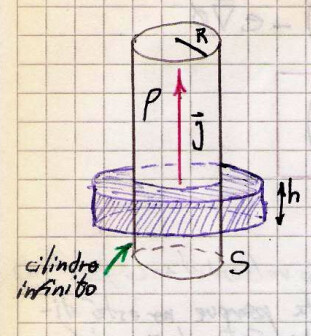
\includegraphics[width=0.4\textwidth]{images/fig_ft1_setup_problema14.jpg}

\[
	\int_S \: \vb{E}\cdot d\vb{S} = 4 \pi Q \qquad \qquad 
	\int_\Gamma \: \vb{B}\cdot d\Bell = \frac{ 4 \pi }{c} I_c
\]
Los campos serán
\[
	2 \pi r h E = 4 \pi 
	\begin{cases}
	\pi R^2 h \rho \quad \rho > R \\ 
	\pi r^2 h \rho \quad \rho < R
	\end{cases}
	\qquad \qquad
	2 \pi r B = \frac{ 4 \pi }{ c }
	\begin{cases}
	\pi R^2 j \quad \rho > R \\ 
	\pi r^2 j \quad \rho < R
	\end{cases}
\]
\[
	\vb{ E } = 
	\begin{cases}
	\frac{ 2 \pi R^2 \rho }{ r^2 } \vbx \quad \rho > R \\ 
	2 \pi \rho \vbx \quad \rho < R
	\end{cases}
	\qquad \qquad
	\vb{B} = 
	\begin{cases}
	\frac{ 2 \pi R^2 }{ c r } j \hat{\theta} \quad \rho > R \\ 
	\frac{ 2 \pi r j }{ c } \hat{\theta} \quad \rho < R
	\end{cases}
\]

Tenemos los invariantes y entonces $\pe{E}{B} \propto \rver\cdot\thetaver $ entonces al final
serán $\vb{E}, \vb{B}$ serán perpendiculares.
\[
	E^2 = \frac{ 4 \pi^2 R^4 \rho^2 }{ r^2 } \qquad B^2 = \frac{ 4 \pi^2 R^4 j^2 }{ c^2 r^2 },
\]
con los campos internos, a menos de un factor dan lo mismo
\[
	E^2 - B^2 = \frac{ 4 \pi^2 R^4 }{ c^2 r^2 } (c^2\rho^2 - j^2),
\]
y el paréntesis es $-j_\mu j^\mu$, que viene de la forma de la cuadricorriente [referir a la primera
vez que aparece]. Se puede hacer esto transformando $\vb{j}$ que lo hace como lo hacen las
coordenadas.

Entonces, los dos casos son $ c \rho > j $ entonces existe sistema $K'$ tal que $\vb{B'}= 0 $.
El otro caso, si $ c \rho < j $ entonces existe sistemas $K'$ tal que $\vb{E'}= 0 $.

En el primer caso se tiene $\vb{B'} = 0 $ y usamos las leyes de transformación de los campos ya
vistas.
\[
	\vb{B'}_\parallel = 0 = \vb{B}_\parallel 
\]
\[
	\vb{B'}_\perp = 0 = \gamma ( \vb{B}_\perp - \pv{\beta}{E} )
\]
y de acá despejamos el campo magnético perpendicular. Entonces $ \vb{B} = \pv{\beta}{E} $.
Habría que ver quién es $\vb{\beta}$, pero las dependencias generales serán
\[
	\vb{B}(\thetaver) = \vb{\beta}(\rver,\zver) \times \vb{E}(\rver),
\]
entonces serán $ \vb{\beta} = \beta \zver $. No pueden tener componente en $\rver$ porque
la velocidad cambiaría punto a punto, entonces sólo en $\zver$.
Finalmente,
\[
	\beta = \frac{ j }{ c \rho },
\]
así se anula $\vb{B}$.

En el segundo caso hay un sistema donde $\vb{E'} = 0$,
\[
	\begin{cases}
	{E'}_\parallel = 0 = \vb{E}_\parallel \\
	{E'}_\perp = 0 = \gamma ( E_\perp + \vb{\beta} \times \vb{B} ) 
	\end{cases}
\]
de lo cual deducimos que $ E_{\parallel} = 0 $ y $ E_\perp = \vb{B} \times \vb{\beta} $,
entonces $ \vb{\beta} = \beta \zver $.
Finalmente,
\[
	\beta = \frac{ c \rho }{ j },
\]
que es el resultado que habíamos obtenido antes.
Los otros campos serán
\[
	\vb{B'} = 0 \qquad \vb{E'} = ?
\]
\[
	\vb{E'}_\parallel = \vb{E}_\parallel = E_z \zver = 0
\]
\[
	\vb{E'}_\perp = \vb{E'} = \gamma ( \vb{E}_\perp + 1/(c\rho) \pv{J}{B} ) 
\]
pero hay que pasar de $r \to r'$.
 
\end{ejemplo}

\begin{ejemplo}{\bf Problema 18 \& 17}

\[
	\begin{cases}
	\frac{\partial \vb{p}}{\partial t} = q ( \vb{E} + \pv{\beta}{B} ) \\
	\dtot{U}{t} = q c \pe{\beta}{E}
	\end{cases}
	\qquad \qquad 
	\begin{cases}
	$\vb{p}$ = m \gamma $\vb{v}$ = m \gamma c $\vb{\beta}$ \\
	U = \gamma m c^2 
	\end{cases}
\]
Para campo eléctrico $\vb{E}$ constante, $\vb{B}=0$ entonces 
\[
	\dtot{\vb{p}}{t} = q \vb{E} 
\]
y tomando la cuenta $\vb{p} - \vb{p}_0 = q \vb{E} \Delta t $, con $\vb{p} = p_0\yver$
y $\vb{E} = E\xver t$.

Entonces,
\[
	p^2 = \frac{ m^2 c^2 \beta^2 }{ 1 - \beta^2 } = p_0^2 + q^2 E^2 t^2
\]
y desarrollando
\[
	1 - \beta^2 = \frac{ m^2 c^2 }{ m^2 c^2 + p_0^2 + q^2 E^2 t^2 }
\]
de lo cual
\[
	\vb{\beta} = \frac{ q \vb{E} t + \vb{p}_0 }{ ( q^2 E^2 t^2 + p_0^2 + m^2 c^2 )^{1/2} }
	\qquad 
	\vb{v} = \frac{ c q \vb{E} t + \vb{p}_0 }{ ( q^2 E^2 t^2 + p_0^2 + m^2 c^2 )^{1/2} }
\]
si definimos el argumento de la raíz que aparece en el denominador, se tienen
\[
	v_z= 0 
	\qquad 
	v_x = \frac{c q E t}{ \sqrt{ \Phi } }
	\qquad 
	v_z = \frac{ p_0 }{ \sqrt{ \Phi } }
\]
 
Ahora integramos estas ecuaciones y obtenemos
\[
	x = c \sqrt{ t^2 + (p_0^2 + m^2 c^2) / q^2 E^2} - \frac{U_0}{qE}
\]
donde la energía inicial es $U_0 = \sqrt{ c^2p_0^2 + m^2c^4 }$, 
\[
	x = \sqrt{ c^2t^2 + \frac{U_0}{q^2E^2} } -  \frac{U_0}{qE}
\]

Para valores de velocidad
\[
	v_y = \frac{ c p_0 }{ q E \sqrt{ t^2 + \alpha^2 } }
\]
con $ \alpha^2 = U_0^2/( c^2 q^2 E^2 )$ y con integración elemental llegamos a
\[
	y = \frac{ c p_0 }{ q E } \asinh\Frac{ c q t E }{U_0}
\]
y correspondientemente
\[
	x = \frac{ U_0 }{ q E }\left[ \cosh\Frac{ q E y }{ c \rho_0 } - 1 \right]
\]
Esto es una especie de parábola.

Para el problema 18 es $\vb{B} = cte.$ y $\vb{E}=0$ 
\[
	\begin{cases}
	\displaystyle \frac{d\vb{p}}{dt} = q \pv{\beta}{B} \\
	\\
	\displaystyle \dtot{U}{t} = 0
	\end{cases}
\]
de lo cual extraemos $ \gamma m c^2 = cte. $. Por otra parte
\[
	\vb{\omega} = \frac{q}{\gamma m c}\vb{B}
\]
y entonces $ \partial \vb{\beta} / \partial t = \pv{\beta}{\omega} $.
Luego,
\[
	\dtot{\vb{\beta}_\parallel}{t} = 0 \qquad \qquad
	\dtot{\vb{\beta}_\perp}{t} = \pv{\beta_\perp}{\omega}
\]
y el campo $ \vb{\beta}_\perp $ sólo varía su dirección, mientras que $\vb{\beta}_\parallel$
es constante. De todo esto saldrá que $\theta = \omega t$.

Se tiene
\[
	\vb{v}_\perp = \omega a ( \cos(\omega\Delta t) \xver + \sin(\omega\Delta t)\yver ),
\]
y el radio de giro es
\[
	a = \frac{ c p_\perp }{ q B },
\]
donde $ v_\perp = \omega a $ de modo que $\beta_\perp = \omega a / c $ y entonces
\[
	p_\perp = \gamma m c \beta_\perp,
\]
lo cual nos provee el link para calcular el radio de giro.
 
\end{ejemplo}

\begin{ejemplo}{\bf Problema 19}

La idea es moverme a un sistema de referencia donde uno se anula y entonces evalúo el otro
(campo en un campo eléctrico o magnético puro). Esto lo puedo hacer si $E \neq B$.

\end{ejemplo}


% \bibliographystyle{CBFT-apa-good}	% (uses file "apa-good.bst")
% \bibliography{CBFT.Referencias} % La base de datos bibliográfica

\end{document}
